\chapter{Revisión Bibliográfica}
\label{chap:revision}
Este capítulo establece las bases teóricas de nuestra investigación, proporcionando un análisis exhaustivo de la literatura existente sobre los tipos de datos, la privacidad de los datos y la generación de datos sintéticos. El objetivo es establecer un contexto para la investigación y una base para el desarrollo de las metodologías aplicadas en los capítulos siguientes.
\section{Tipos de Datos}
\label{tipo-de-datos}
Los tipos de datos tienen diversas implicaciones en su generación, como su representación, almacenamiento y procesamiento. Los datos estructurados se presentan en la Tabla \ref{tabla-tipo-datos}.

En 2012, IDC estimó que para 2020, más del 95\% de los datos serían no estructurados \cite{gantz_digital_2012}. En un análisis posterior, Kiran Adnan y Rehan Akbar \cite{adnan_analytical_2019} encontraron que el texto es el tipo de dato no estructurado que más rápido crece en las publicaciones, seguido por la imagen, el video y finalmente el audio.

La Tabla \ref{tabla-tipo-datos} resume la lista que se encuentra en \emph{Practical Statistics for Data Scientists} \cite{bruce_practical_2020}.

\begin{table}[H]
	\centering
	\caption{Tipos de datos estructurados}
	\label{tabla-tipo-datos}
    \begin{tabular}{|l|l|m{20em}|m{9em}|}
    \hline
    \rowcolor[gray]{0.8}
    T & Sub tipo & Descripción & Ejemplos \\
    \hline
    \multicolumn{2}{|>{\columncolor[gray]{0.8}}c|}{Numérico} & Datos establecidos como números & \cellcolor[gray]{0.8} - \\
    \hline
    \cellcolor[gray]{0.8} & Continuo & Datos que pueden tomar cualquier valor en un intervalo & 3.14 metros, 1.618 litros \\
    \hline
    \cellcolor[gray]{0.8} & Discreto & Datos que solo pueden tomar valores enteros & 1 habitación, 73 años \\
    \hline
    \multicolumn{2}{|>{\columncolor[gray]{0.8}}c|}{Categórico} & Datos que pueden tomar solo un conjunto específico de valores que representan un conjunto de categorías posibles. & \cellcolor[gray]{0.8} - \\
    \hline
    \cellcolor[gray]{0.8} & Binario & Un caso especial de datos categóricos con solo dos categorías de valores & 0/1, verdadero/falso \\
    \hline
    \cellcolor[gray]{0.8} & Ordinal & Datos categóricos que tienen un ordenamiento explícito. & pequeña/ mediana/ grande \\
    \hline
    \end{tabular}
\end{table}

\section{Privacidad de Datos}
La protección de la información es un aspecto fundamental en la generación de datos sintéticos. Aunque este aspecto puede no ser crucial cuando los datos corresponden a temas como recetas o automóviles, resulta esencial cuando se trata de información relacionada con individuos \cite{bruce_practical_2020}. Por esta razón, el resguardo de la información es un tema de importancia para entidades como Equifax, que gestionan una gran cantidad de conjuntos de datos con contenido personal.

\subsection{Tipo de datos a ser protegidos}
Para identificar qué campos de datos son significativos desde el punto de vista de la privacidad, se puede recurrir a la definición resumida en la Tabla \ref{data-relevante} del texto \emph{Data privacy: Definitions and techniques} \cite{de_capitani_di_vimercati_data_2012}.

\begin{table}[H]
	\centering
	\caption{Niveles de revelación y ejemplos}
	\label{data-relevante}
    \begin{tabular}{|m{15em}|m{20em}|}
    \hline
    \rowcolor[gray]{0.8}
    Tipo de revelación & Descripción \\
    \hline
    \textbf{Identificadores} 
    & Atributos que identifican de manera única a individuos (por ejemplo, SSN, RUT, DNI). \\
    \hline
    \textbf{Cuasi-identificadores (QI)} 
    & Atributos que, en combinación, pueden identificar a individuos, o reducir la incertidumbre sobre sus identidades (por ejemplo, fecha de nacimiento, género y código postal). \\
    \hline
    \textbf{Atributos confidenciales} 
    & Atributos que representan información sensible (por ejemplo, enfermedad). \\
    \hline
    \textbf{Atributos no confidenciales} 
    & Atributos que los encuestados no consideran sensibles y cuya divulgación es inofensiva (por ejemplo, color favorito). \\
    \hline
    \end{tabular}
\end{table}

\subsection{Tipos de riesgos de divulgación}
Los tipos de divulgación definidos en \emph{Practical Synthetic Data Generation} \cite{bruce_practical_2020} están resumidos en la Tabla \ref{relevantes-definiciones}.

\begin{table}[H]
	\centering
	\caption{Tipos de Riesgos de Divulgación y sus Descripciones}
	\label{relevantes-definiciones}
    \begin{tabular}{|m{15em}|m{20em}|}
    \hline
    \rowcolor[gray]{0.8}
    Tipo de revelación & Descripción \\
    \hline
    \textbf{Divulgación de identidad} 
    & Este riesgo se refiere a la posibilidad de que un atacante pueda identificar la información de un individuo a partir de los datos publicados, utilizando técnicas de filtrado para reducir las posibilidades hasta un solo individuo.\\
    \hline
    \textbf{Divulgación de nueva información} 
    & Este riesgo comprende el riesgo de Divulgación de Identidad, y además, implica la adquisición de información adicional sobre el individuo a partir de los datos publicados.\\
    \hline
    \textbf{Divulgación de Atributos} 
    & Este riesgo se da cuando, aunque no se pueda identificar a un individuo, se puede descubrir un atributo común en varios registros, lo que permite obtener información sensible acerca de un grupo de individuos.\\
    \hline
    \textbf{Divulgación Inferencial} 
    & Este riesgo se refiere a la posibilidad de inferir información sensible a partir de los datos publicados, mediante el uso de técnicas de análisis estadístico o de aprendizaje automático. Por ejemplo, si después de filtrar todos los registros, el 80\% de los registros con las mismas características tienen cáncer, se podría inferir que el individuo buscado puede tener cáncer.\\
    \hline
    \end{tabular}
\end{table}


Adicionalmente se deben establecer dos conceptos relevantes ante el análisis de revelación de información:
\begin{enumerate}
    \item En términos prácticos, normalmente los datos sintéticos buscan tener cierta permeabilidad con respecto a la \textbf{Divulgación Inferencial}, ya que se quiere que estadísticamente sean similares. Además, se busca proteger la identidad de los individuos, pero esta no es la única condición, también se busca proteger aquellos atributos que pueden ser sensibles, como las enfermedades. A todo este conjunto se le denomina \textbf{Revelación de identidad significativa}. Es particularmente riesgoso por la posibilidad de discriminación hacia ciertos grupos que cumplen con los atributos criterio.
    \item Los mismos atributos pueden tener más relevancia para ciertos grupos de la población que para otros. El ejemplo que se indica en \cite{el_emam_practical_2020} es que, debido a que el número de hijos igual a 2 es menos frecuente en una etnia que en otra (40\% en la primera y 10\% en la segunda), ese dato es más relevante en la segunda. Esto se debe a que es un factor que filtra mejor y, por lo tanto, puede permitir un mejor conocimiento de ese grupo específico. A esto se le denomina \textbf{Definición de información ganada}.
\end{enumerate}

\subsection{Regulación de datos sintéticos}
Debido a que los datos sintéticos son basados en datos reales, pueden ser afectos a las regulaciones de sobre protección de datos \cite{bruce_practical_2020}. Los nuevos datos podrían ser afectos por:
\begin{enumerate}
    \item \href{https://dvbi.ru/Portals/0/DOCUMENTS_SHARE/RISK_MANAGEMENT/EBA/GDPR_eng_rus.pdf}{Regulation (EU) 2016/679 of the European Parliament and of the Council} \cite{regulation_regulation_2016}, si el proceso de generación de datos sintéticos a menudo implica el uso de datos personales reales como entrada. En este caso, el GDPR sería relevante. Las organizaciones que utilicen datos personales para generar datos sintéticos deben garantizar que este proceso cumple con los principios del GDPR, como la minimización de datos (sólo se deben utilizar los datos necesarios) y la limitación de la finalidad (los datos sólo se deben utilizar para el propósito para el que se recogieron).
    \item \href{https://heinonline.org/HOL/LandingPage?handle=hein.journals/jtlp23&div=5&id=&page=}{The California consumer privacy act: Towards a European-style privacy regime in the United States} \cite{pardau_california_2018}
    \item \href{http://www.eolusinc.com/pdf/hipaa.pdf}{Health insurance portability and accountability act of 1996} \cite{act_health_1996}
\end{enumerate}

\section{Generación de Datos Sintéticos}

Los datos sintéticos, aunque no son datos reales, se generan con la intención de preservar ciertas propiedades de los datos originales. La utilidad de los datos sintéticos se mide por su capacidad para servir como un sustituto efectivo de los datos originales \cite{bruce_practical_2020}. Basándose en el uso de los datos originales, los datos sintéticos se pueden clasificar en tres categorías: aquellos que se basan en datos reales, los que no se basan en datos reales, y los híbridos.

\begin{itemize}
    \item \textbf{Datos basados en datos reales}: utilizan modelos que aprenden la distribución de los datos originales para generar nuevos puntos de datos similares.
    \item \textbf{Datos no basados en datos reales}: utilizan conocimientos del mundo real. Por ejemplo, se podría formar un nombre completo seleccionando aleatoriamente un nombre y un apellido de un conjunto predefinido.
    \item \textbf{Híbridos}: estos combinan técnicas de imitación de distribución con algunos campos que no derivan de los datos reales. Esto puede ser especialmente útil cuando se intenta desacoplar las distribuciones de datos que podrían ser sensibles o generar discriminación, como la información sobre la etnia.
\end{itemize}
    
En la Tabla \ref{tipo-de-datos}, se revisaron los datos estructurados. Si bien cada tipo puede tener muchas representaciones, por ejemplo, los datos continuos podrían considerarse como \emph{float}, \emph{datetime} o incluso intervalos personalizados, como de 0 a 1. Sobre estos datos estructurados, se pueden generar estructuras para unirlos.

Entre las estructuras más comunes se encuentran las matrices bidimensionales (datos tabulares) y los arreglos, que permiten matrices de muchas dimensiones e incluso estructuras complejas que pueden mezclar todas las estructuras previas.

Debido al objetivo, se detallan solo los modelos que permiten abordar la generación de datos tabulares y texto basados en datos reales.
\subsection{Generación de datos tabulares}
En la Tabla \ref{tab-sota-tab}, se resumen las últimas publicaciones sobre generación de datos tabulares, indicando la fecha de publicación y si se puede acceder al código fuente o no, a febrero de 2023.

\begin{table}[H]
	\centering
	\caption{Estado del arte en generación de datos tabulares}
	\label{tab-sota-tab}
    \begin{tabular}{|m{28em}|r|r|}
    \hline
    \rowcolor[gray]{0.8}
    Nombre & Fecha $\downarrow$ & Código \\
    \hline
    REaLTabFormer: Generating Realistic Relational and Tabular Data using Transformers \cite{solatorio_realtabformer_2023}
    & 2023-02-04 & \href{https://github.com/avsolatorio/REaLTabFormer}{Github} \\
    \hline
    PreFair: Privately Generating Justifiably Fair Synthetic Data \cite{pujol_prefair_2022}
    & 2022-12-20 & \\
    \hline
    GenSyn: A Multi-stage Framework for Generating Synthetic Microdata using Macro Data Sources \cite{acharya_gensyn_2022}
    & 2022-12-08 & \href{https://github.com/Angeela03/GenSyn}{Github} \\
    \hline
    TabDDPM: Modelling Tabular Data with Diffusion Models \cite{kotelnikov_tabddpm_2022}
    & 2022-10-30 & \href{https://github.com/rotot0/tab-ddpm}{Github} \\
    \hline
    Language models are realistic tabular data generators \cite{borisov_language_2022}
    & 2022-10-12 & \href{https://github.com/kathrinse/be_great}{Github} \\
    \hline
    Ctab-gan+: Enhancing tabular data synthesis \cite{zhao_ctab-gan_2022}
    & 2022-04-01 & \href{https://github.com/Team-TUD/CTAB-GAN-Plus}{Github} \\
    \hline
    Ctab-gan: Effective table data synthesizing \cite{zhao_ctab-gan_2021}
    & 2021-05-31 & \href{https://github.com/Team-TUD/CTAB-GAN}{Github} \\
    \hline
    Modeling Tabular data using Conditional GAN \cite{xu_modeling_2019}
    & 2019-10-28 & \href{https://github.com/sdv-dev/SDV}{Github} \\
    \hline
    Smote: synthetic minority over-sampling technique \cite{chawla_smote_2002}
    & 2002-06-02 & \href{https://github.com/scikit-learn-contrib/imbalanced-learn}{Github} \\
    \hline
    \end{tabular}
\end{table}


\subsection{Generación de texto en base de datos tabulares}

En la Tabla \ref{tab-sota-text}, se listan las publicaciones en la generación de texto a partir de datos estructurados.

\begin{table}[H]
	\centering
	\caption{Estado del arte en generación de textos en base a datos}
	\label{tab-sota-text}
    \begin{tabular}{|m{20em}|r|r|}
        \hline
        \rowcolor[gray]{0.8}
        Nombre & Fecha $\downarrow$ & Modelo Base \\
        \hline
        Table-To-Text generation and pre-training with TABT5 \cite{andrejczuk_table--text_2022}
        & 2022-10-17
        & T5 \\
        \hline
        Text-to-text pre-training for data-to-text tasks \cite{kale_text--text_2020}
        & 2021-07-09
        & T5 \\
        \hline
        TaPas: Weakly supervised table parsing via pre-training \cite{herzig_tapas_2020}
        & 2020-04-21
        & Bert \\
        \hline
    \end{tabular}
\end{table}

El estado del arte en la generación de texto a partir de datos tabulares es TabT5. Es importante notar que la tabla mezcla los enfoques de \emph{Table-To-Text} y \emph{Data-To-Text}. Aunque ninguna de las publicaciones incluye código asociado, no es necesario, ya que utilizan modelos abiertos como base (T5 y Bert). Lo más relevante en estos casos es el proceso de \emph{fine-tuning}. Para completar la tarea de generar nuevos textos a partir de información inicial, esta información debe ser codificada para poder ser procesada por el modelo utilizado.

La diferencia entre \emph{Table-To-Text} y \emph{Data-To-Text} radica en el formato de información de entrada. en \emph{Table-To-Text} es una tabla con multiples filas y en \emph{Data-To-Text} corresponde a un solo objeto con sus propiedades. A continuación ejemplos de entradas de los modelos.


En los siguientes ejemplos, se utilizará la Tabla \ref{tabla-ejemplo-inputs} para ilustrar cómo se puede utilizar para generar texto utilizando los modelos de \emph{fine-tuning} mencionados anteriormente. Esta tabla representa información sobre películas, incluyendo el nombre de la película, el director, el año de lanzamiento y el género, y se utilizará para generar preguntas y respuestas a partir de la información proporcionada.
\begin{table}[H]
	\centering
	\caption{Ejemplo de tabla de entrada}
	\label{tabla-ejemplo-inputs}
    \begin{tabular}{|l|l|l|l|}
        \hline
        \rowcolor[gray]{0.8}
        Nombre de la Película & Director & Año de Lanzamiento & Género \\
        \hline
        Star Wars: Una Nueva Esperanza & George Lucas & 1977 & Ciencia ficción \\
        \hline
    \end{tabular}
        
\end{table}

Para los modelos TabT5 y TaPas, se utiliza el mismo preprocesamiento para convertir la tabla de entrada en una pregunta/tarea y respuesta \cite{andrejczuk_table--text_2022, herzig_tapas_2020}. En este ejemplo, la tabla representa información sobre películas, y se utiliza para generar una pregunta y respuesta sobre el director de la película "Star Wars: Una Nueva Esperanza". La pregunta se construye a partir de la información de la tabla, y la respuesta se espera que sea el nombre del director. Una vez que se ha generado la pregunta y la respuesta, se puede utilizar un modelo de \emph{fine-tuning} como TabT5 o TaPas para generar texto a partir de la información proporcionada. En resumen, el proceso de generación de texto a partir de datos tabulares implica la conversión de información tabular en preguntas y respuestas, y luego la utilización de modelos de \emph{fine-tuning} para generar texto a partir de estas preguntas y respuestas.
\begin{tcolorbox}[colback=white,colframe=black!50!white,title=Input]
Table: Películas
Nombre de la Película     | Director                | Año de Lanzamiento | Género 
Star Wars: Una Nueva Esperanza | George Lucas        | 1977              | Ciencia ficción 
\end{tcolorbox}
\begin{tcolorbox}[colback=white,colframe=black!50!white,title=Pregunta]
¿Qué director dirigió la película Star Wars: Una Nueva Esperanza?
\end{tcolorbox}
\begin{tcolorbox}[colback=white,colframe=black!50!white,title=Respuesta esperada]
George Lucas
\end{tcolorbox}


En cambio, el modelo \emph{Text-to-text pre-training for data-to-text tasks} \cite{kale_text--text_2020} utiliza una entrada diferente, que consiste en una serie de tuplas que representan las propiedades de la entidad y sus valores correspondientes. Se espera que el modelo identifique la tupla relevante y genere una pregunta y respuesta correspondientes. Una vez generada la pregunta y respuesta, se puede utilizar el modelo de fine-tuning correspondiente para generar texto a partir de ellas. En conclusión, la generación de texto a partir de datos tabulares implica una conversión adecuada de la información de entrada en un formato apropiado para cada modelo, la identificación de la pregunta o tarea relevante y la utilización del modelo correspondiente para generar el texto resultante.

\begin{tcolorbox}[colback=white,colframe=black!50!white,title=Input]
<Star Wars: Una Nueva Esperanza, Director, George Lucas>, \\
<Star Wars: Una Nueva Esperanza, Año de Lanzamiento, 1977>, \\
<Star Wars: Una Nueva Esperanza, Género, Ciencia ficción>
\end{tcolorbox}
\begin{tcolorbox}[colback=white,colframe=black!50!white,title=Pregunta]
¿Qué director dirigió la película Star Wars: Una Nueva Esperanza?
\end{tcolorbox}
\begin{tcolorbox}[colback=white,colframe=black!50!white,title=Respuesta esperada]
George Lucas
\end{tcolorbox}


\section{Metricas de evaluación}
Es importante destacar que no todas estas métricas son aplicables a todos los tipos de datos y modelos, y que la selección de las métricas a utilizar debe ser cuidadosamente considerada en función de las necesidades y objetivos específicos de cada caso de estudio.
A continuación presentan algunas de las posibles a considerar para medir la similitud, privacidad y utilidad en la evaluación de los conjuntos de datos sintéticos generados.
\begin{itemize}
\item \textbf{SDMetrics Score}: Este es un promedio de las métricas de 'Quality Report' y 'Diagnostic Report' que varían de 0 a 1. El 'Quality Report' se refiere a las formas de las columnas (Column Shapes) y las tendencias entre pares de columnas (Column Pair Trends). El 'Diagnostic Report' se refiere a la síntesis (Synthesis), cobertura (Coverage) y límites (Boundaries).
\item \textbf{Reporte diagnóstico}: Se refiere a un conjunto de métricas que incluyen Síntesis, Cobertura y Límites. La síntesis verifica la singularidad de los datos sintéticos, la cobertura verifica si los datos sintéticos cubren todo el espectro de valores y los límites verifican si los datos sintéticos respetan los límites de los datos reales.
\item \textbf{Reporte de calidad}: En este informe se revisan dos componentes, las formas de las columnas (Column Shapes) y las tendencias entre pares de columnas (Column Pair Trends). La forma de las columnas mide la capacidad de los datos sintéticos para capturar la distribución general de cada columna en los datos reales. Las tendencias entre pares de columnas describen cómo varían en relación entre sí.
\item \textbf{Correlación}: En esta sección se utiliza la correlación de Pearson en columnas numéricas para generar una representación visual en un mapa de calor.
\item \textbf{Privacidad}: Esta sección cubre dos métricas, Distancia al Registro más Cercano (DCR) y Relación de Distancia del Vecino más Cercano (NNDR). DCR cuantifica la distancia euclidiana entre cualquier registro sintético y su vecino real más cercano. NNDR mide la relación entre la distancia euclidiana al vecino real más cercano y al segundo vecino real más cercano de cualquier registro sintético.
\item \textbf{Propiedades estadísticas}: Esta sección presenta un conjunto de propiedades estadísticas como el número de observaciones, elementos faltantes, media, mediana, moda, entre otros.
\end{itemize}




\subsection{SDMetrics Score}
En la Tablas incluidas en la sección \emph{SDMetrics Score} se expresa en su última columna un promedio de \emph{Quality Report} de SDMetric. Adicionalmente se incluyen las metricas calculadas en \emph{Diagnostic Report}. Todas las metricas expresadas en este apartado van del 0 al 1, ya que las métricas promediadas van en este rango tambien. Detalles de cada metricas se podrán encontrar en las siguientes subsecciones \ref{Diagnostic Report} y \ref{Quality Report}.
\[
    Score = \frac{\text{Column Pair Trends}+\text{Column Shapes}}{2}
\]
El \emph{Quality Report} captura las formas de las columnas (\emph{Column Shapes}) y las tendencias entre pares de columnas (\emph{Column Pair Trends}). La forma de una columna describe su distribución general, y la tendencia entre dos columnas describe cómo varían en relación entre sí. Es importante tener en cuenta que las distribuciones de orden superior de 3 o más columnas no se incluyen en el \emph{Quality Report}. Detalles de cada métricas se podrán encontrar en Sección \ref{Quality Report}.

Por otro lado, el \emph{Diagnostic Report} mide la síntesis (\emph{Synthesis}), cobertura (\emph{Coverage}) y límites (\emph{Boundaries}). La síntesis se refiere a si los datos sintéticos son únicos o si copian las filas reales. La cobertura verifica si los datos sintéticos cubren el rango de valores posibles. Los límites, por su parte, comprueban si los datos sintéticos respetan los límites establecidos por los datos reales. Al igual que en el \emph{Quality Report}, se aplican métricas basadas en los tipos de columnas y se promedian para obtener una puntuación final. Detalles de cada métricas se podrán encontrar en Sección \ref{Diagnostic Report}.

\begin{table}[H]
    \centering
    \fontsize{10}{14}\selectfont
    \caption{Ejemplo de Métricas de Rendimiento para Diversos Modelos}
    \label{example-table-score}
    \begin{tabular}{|l|r|r|r|r|r|r|}
    \hline
    \rowcolor[gray]{0.8}
    Model Name & Column Pair Trends & Column Shapes & Coverage & Boundaries & Synthesis & \textbf{Score} \\
    \hline tddpm\_mlp & \bfseries 9.73e-01 & \bfseries 9.84e-01 & \bfseries 7.91e-01 & \bfseries 1.00e+00 & 9.91e-01 & \bfseries 9.79e-01 \\
    \hline smote-enc & 9.62e-01 & 9.76e-01 & 6.67e-01 & \bfseries 1.00e+00 & 9.24e-01 & 9.69e-01 \\
    \hline copulagan & 7.46e-01 & 7.90e-01 & 6.80e-01 & \bfseries 1.00e+00 & \bfseries 1.00e+00 & 7.68e-01 \\
    \hline
    \end{tabular}
\end{table}




\subsection{Reporte diagnóstico}
\label{Diagnostic Report}
La evaluación se lleva a cabo mediante una serie de métricas que se agrupan en: \emph{Synthesis}, \emph{Coverage}, y \emph{Boundaries}.

\emph{Synthesis} emplea \emph{NewRowSynthesis} en SDMetrics, la cual verifica la singularidad de los datos sintéticos, esto es, si los datos sintéticos copian filas completas de los datos reales o si son capaces de generar nuevas filas únicas. Para su cálculo, en primer lugar, se obtiene un conjunto único de filas tanto para los datos reales como para los sintéticos. Posteriormente, se calcula el número de filas únicas que se encuentran en los datos sintéticos pero no en los reales. Finalmente, este número se divide por el número total de filas únicas en los datos sintéticos para obtener la probabilidad de generar una nueva fila única. En lo que respecta a la puntuación, un valor de 1.0 indica que todos los datos sintéticos y reales son idénticos, mientras que un valor de 0.0 señala que todos los datos sintéticos y reales son completamente diferentes.

La métrica \emph{RangeCoverage} se emplea para determinar si una columna sintética cubre todo el espectro de valores presentes en una columna real. Esta métrica es compatible con datos numéricos continuos y de tiempo/fecha, los cuales se transforman en valores numéricos. Los valores vacíos son ignorados por esta métrica. El cálculo de la puntuación se realiza de acuerdo con la siguiente fórmula, donde \(r\) y \(s\) representan las columnas real y sintética respectivamente:

\[
\text{{score}} = 1 - \left[ \max\left(\frac{{\min(s) - \min(r)}}{{\max(r) - \min(r)}}, 0\right) + \max\left(\frac{{\max(r) - \max(s)}}{{\max(r) - \min(r)}}, 0\right) \right]
\]

La métrica \emph{Boundaries} se emplea para evaluar si una columna sintética respeta los valores mínimos y máximos de la columna real, devolviendo el porcentaje de filas sintéticas que se mantienen dentro de los límites reales. Esta métrica se aplica a los datos numéricos, transformando los valores de fecha y hora en valores numéricos, e ignorando los valores ausentes. Un valor de 0.9 en esta métrica significa que el 10\% de los registros no respeta los límites de los datos reales.




\subsection{Reporte de calidad}
\label{Quality Report}

El \emph{Quality Report} en SDMetrics consta de dos componentes principales: \emph{Column Shapes} y \emph{Column Pair Trends}. Existe un tercero, pero que solo se útiliza cuando se genera varios conjuntos de datos relacionados.

El primero, \emph{Column Shapes}, mide la capacidad de los datos sintéticos para capturar la forma de cada columna en los datos reales. La forma de una columna describe su distribución general. Para realizar esta evaluación, se utilizan dos métricas basadas en los tipos de dato de la columna. Por ejemplo, para las columnas numéricas y de fecha y hora, se utiliza la métrica \emph{KSComplement}, mientras que para las columnas categóricas y booleanas, se utiliza la métrica \emph{TVComplement}.

El \emph{KSComplement} utiliza la estadística de Kolmogorov-Smirnov para calcular la similitud entre las columnas reales y sintéticas. En particular, se convierte la distribución numérica en su función de distribución acumulativa, CDF por sus siglas en ingles de \emph{Cumulative distribution function}, y la estadística de KS es la diferencia máxima entre las dos CDFs. En SDMetrics, se invierte la estadística: \emph{KSComplement} devuelve $1 - (\text{estadística de KS})$ para que una puntuación más alta signifique una mayor calidad. En la Figura \ref{sdmetric_cdf} se puede observar una representación grafica del calculo.


\begin{figure}[H] 
    \centering
    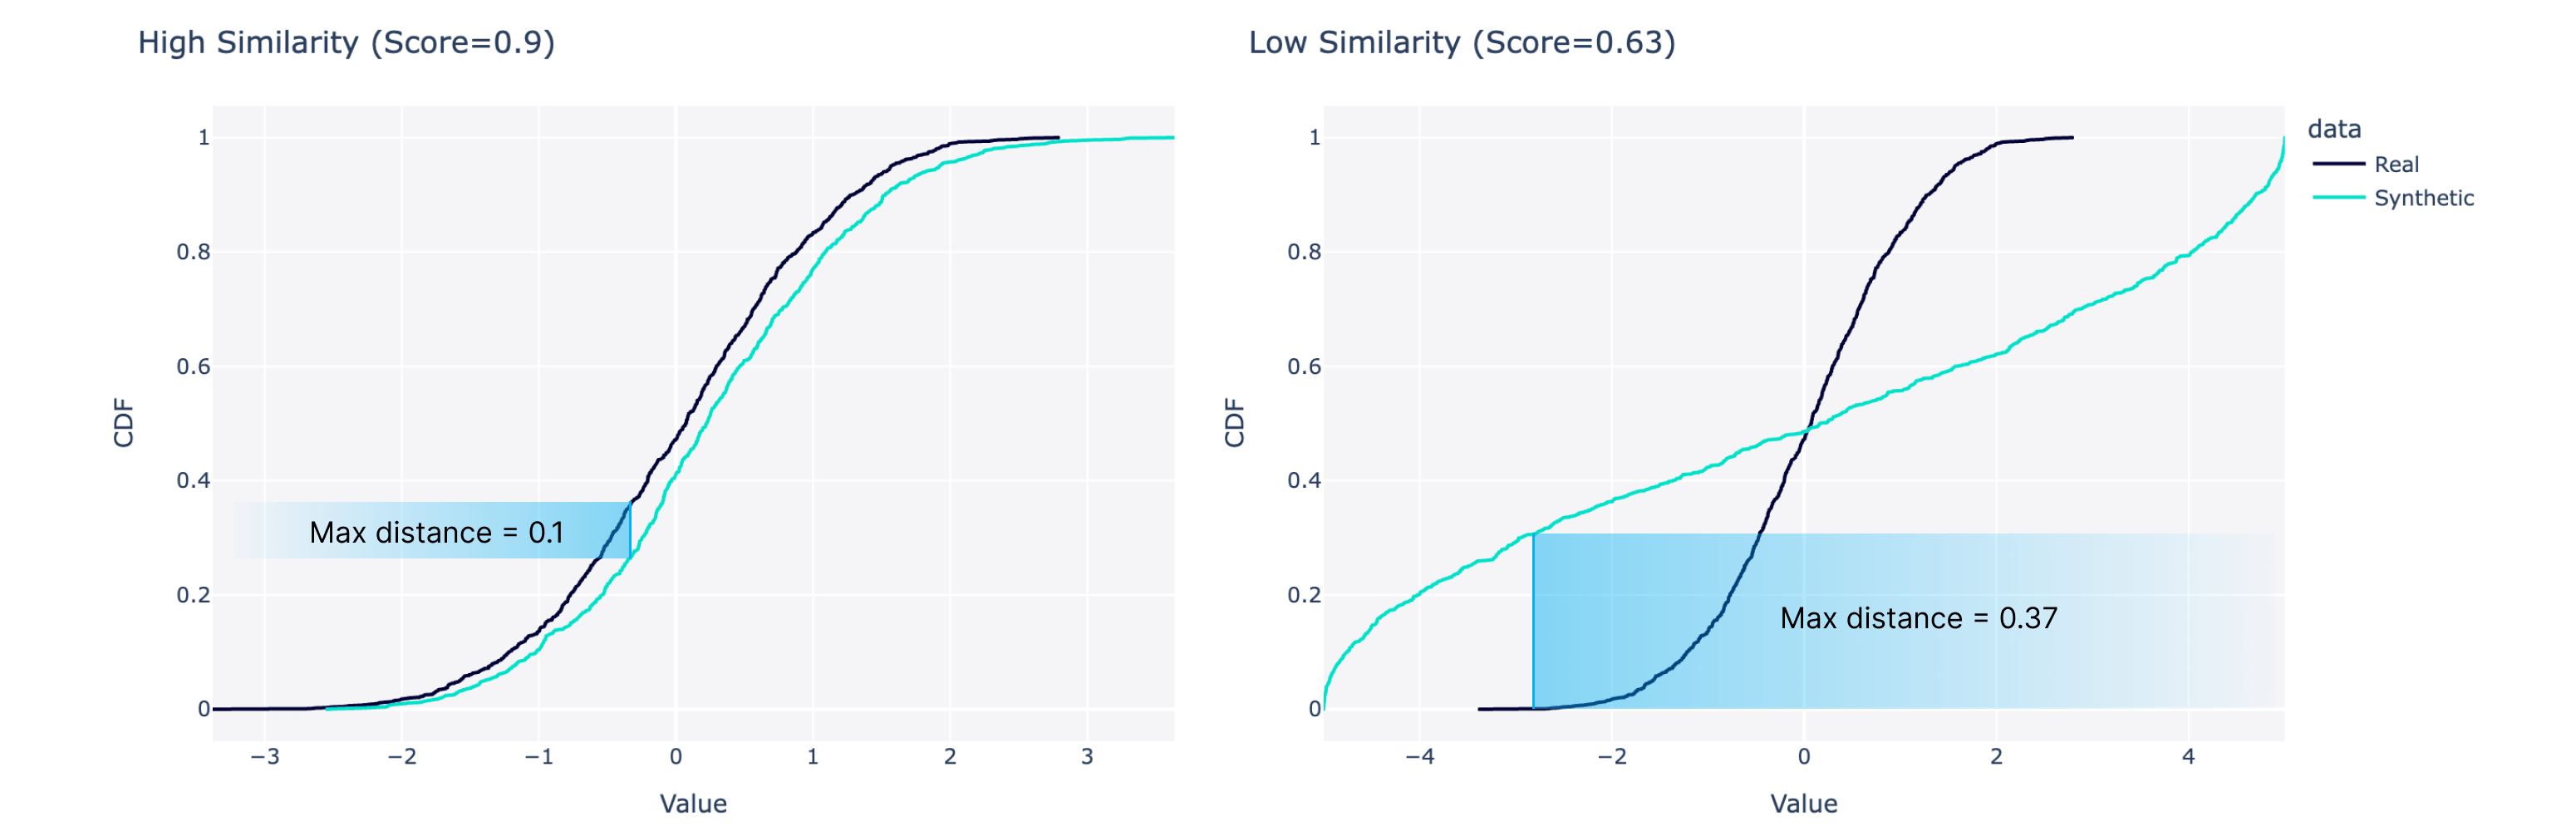
\includegraphics[width=.7\textwidth]{imagenes/SDMetrics/KSComplement_Description.png} 
    \caption{Ejemplo de SDMetric en calculo de CDF \cite{noauthor_synthetic_nodate}}
    \label{sdmetric_cdf} % puedes referirte a la imagen en tu documento usando \ref{fig:my_label}
\end{figure}

\emph{TVComplement} calcula la distancia de variación total, conocida como TVD por su acrónimo en inglés de \emph{Total Variation Distance}, entre las columnas reales y sintéticas. Para lograr esto, en primer lugar estima la frecuencia de cada valor de categoría y la expresa en términos de probabilidad. La estadística TVD compara las diferencias en estas probabilidades, siguiendo la fórmula:
\[
\delta(R,S) = 2 \sum_{\omega \in \Omega} |R_\omega - S_\omega|
\]
Aquí, $\omega$ representa todas las posibles categorías en una columna, $\Omega$. Por otro lado, $R$ y $S$ hacen referencia a las frecuencias reales y sintéticas para dichas categorías, respectivamente. \emph{TVComplement} retorna $1 - \text{TVD}$ de modo que una puntuación más alta denote una calidad superior.

\emph{CorrelationSimilarity} es una métrica únicamente aplicable a variables numéricas; las fechas son transformadas a números para este fin. Esta métrica calcula la correlación utilizando los coeficientes de Pearson y Spearman. El score se obtiene mediante la siguiente fórmula, donde $S_{A,B}$ representa la correlación del conjunto sintético y $R_{A,B}$ la correlación del conjunto real.
\[
score = 1 - \frac{|S_{A,B} - R_{A.B}|}{2}
\]


\subsection{Correlación}
En esta sección, se emplea la métrica de correlación de Pearson en las columnas numéricas, transformando las fechas en números e ignorando los valores ausentes, con el propósito de generar una representación visual en un mapa de calor para su análisis.


\subsection{Privacidad}
La Distancia al Registro más Cercano (DCR, por sus siglas en inglés) se emplea para cuantificar la distancia euclidiana entre cualquier registro sintético y su vecino real más próximo. Idealmente, a medida que la DCR se incrementa, el riesgo de violación de la privacidad disminuye. Adicionalmente, se estima el percentil 5 de esta métrica para proporcionar una medición robusta del riesgo de privacidad \cite{zhao_ctab-gan_2021}.

Relación de Distancia del Vecino más Cercano (NNDR, por sus siglas en inglés). La NNDR mide la relación entre la distancia euclidiana para el vecino real más cercano y el segundo vecino real más cercano a cualquier registro sintético correspondiente. NNDR es un concepto comúnmente utilizado en el área de visión por computadora para el emparejamiento de descriptores de imagen locales. Platzer \cite{noauthor_virtual_2022} introduce esta idea para evaluar la privacidad de los datos sintéticos. Esta relación está dentro del intervalo [0, 1]. Valores más altos indican una mejor privacidad. Los valores bajos de NNDR entre datos sintéticos y reales pueden revelar información sensible del registro de datos reales más cercano. La Fig. 6 ilustra el caso. Tenga en cuenta que también se calcula aquí el percentil 5 \cite{zhao_ctab-gan_2021}.


\subsection{Propiedades estadísticas y tecnicas de analizis}

\begin{longtable}{|m{7em}|m{5em}|m{20em}|}
    \caption{Listado de conjunto estadísticos} 
    \label{tab-stats} \\
    \hline
    \rowcolor[gray]{0.8}
    Nombre & abrev. & Descripción \\
    \hline
    \endfirsthead
    
    \hline
    \rowcolor[gray]{0.8}
    Nombre & abrev. & Descripción \\
    \hline
    \endhead
    
    \hline \multicolumn{2}{|r|}{{Continúa en la siguiente página}} \\ \hline
    \endfoot
    
    \hline \hline
    \endlastfoot
    \hline
    Numero de observaciones & nobs & Cuenta de elementos \\
    \hline
    Vacios & missing & Numero de elementos vacios \\
    \hline
    Media & mean & La suma de todos los valores dividido por el número total de valores \\
    \hline
    Mediana & median & El valor que se encuentra en el centro de un conjunto de datos ordenados de menor a mayor. Es decir, la mitad de los valores son mayores que la mediana y la otra mitad son menores \\
    \hline
    Moda & mode & El valor que aparece con mayor frecuencia en un conjunto de datos \\
    \hline
    Mínimo & min & El valor más pequeño en un conjunto de datos \\
    \hline
    Máximo & max & El valor más grande en un conjunto de datos \\
    \hline
    Percentil & 0.1\%, ... 99.9\% & El valor tal que P (25 o 75) por ciento de los datos son menores que él, y el restante (100 - P) por ciento son mayores. Cuando P = 50, el percentil es la mediana \\
    \hline
    Media Truncada & tmean & El promedio de todos los valores, una vez que se han eliminado un porcentaje de los valores más bajos y un porcentaje de los valores más altos \\
    \hline
    Varianza & var & La medida de cuán dispersos están los valores en un conjunto de datos. Es la suma de los cuadrados de las desviaciones desde la media dividido por n - 1, donde n es el número de valores \\
    \hline
    Desviación Estándar & std & La raíz cuadrada de la varianza \\
    \hline
    Error estándar de la media & std\_err & Medida de la variación de las muestras de la media poblacional. \\
    \hline
    Desviación Absoluta Media & mad & La media de los valores absolutos de las desviaciones desde la media \\
    \hline
    Desviación Mediana Absoluta Normalizada & mad\_normal & Medida de dispersión basada en la mediana que normaliza la desviación mediana absoluta utilizando la constante de escala 1.4826 para la distribución normal. \\
    \hline
    Rango & range & La diferencia entre el valor más grande y el valor más pequeño en un conjunto de datos \\
    \hline
    Tablas de Frecuencia & top5\_freq & Un método para resumir los datos al contar cuántas veces ocurre cada valor en un conjunto de datos \\
    \hline
    Probabilidad & top5\_prob & La medida de la posibilidad de que un evento ocurra. Se establece como el número de ocurrencias de un valor dividido por el número total de ocurrencias \\
    \hline
    Tabla de Contingencia & cont\_table & Una tabla que muestra la distribución conjunta de dos o más variables categóricas \\
    \hline
    Comparación de Modelos Predictivos Multivariables & cross\_pred & Un método para comparar varios modelos predictivos que involucran múltiples variables. Implica la construcción de modelos separados para cada variable objetivo y comparar la curva ROC (Receiver Operating Characteristic) para cada modelo \\
    \hline
    Kullback-Leibler & kl & Una medida de la divergencia entre dos distribuciones de probabilidad \\
    \hline
    Log-Cluster & log\_cluster & Un método para evaluar la calidad de los conjuntos de datos sintéticos que compara la estructura de los conjuntos de datos reales y sintéticos mediante el uso de clustering \\
    \hline
    Cross-Classification & cross\_class & Un método para evaluar la calidad de los conjuntos de datos sintéticos que compara la precisión de los modelos predictivos construidos a partir de los conjuntos de datos reales y sintéticos \\
    \hline
    Intervalo de confianza superior & upper\_ci & Valor máximo del intervalo de confianza alrededor de la media. \\
    \hline
    Intervalo de confianza inferior & lower\_ci & Valor mínimo del intervalo de confianza alrededor de la media. \\
    \hline
    Rango intercuartil & iqr & Diferencia entre el tercer y el primer cuartil, mide la dispersión de los datos. \\
    \hline
    Rango intercuartil normalizado & iqr\_normal & Rango intercuartil dividido por la media, para normalizar los valores. \\
    \hline
    Coeficiente de variación & coef\_var & Relación entre la desviación estándar y la media, mide la dispersión relativa de los datos. \\
    \hline
    Sesgo & skew & Medida de la asimetría de la distribución de los datos alrededor de la media. \\
    \hline
    Curtosis & kurtosis & Medida de la "pesadez" de las colas de la distribución de los datos. \\
    \hline
    Test de Jarque-Bera & jarque\_bera & Estadístico que mide si los datos tienen la asimetría y la curtosis correspondiente a una distribución normal. \\
    \hline
    p-valor del test de Jarque-Bera & jarque\_bera \_pval & Probabilidad de que los datos sean normalmente distribuidos según el test de Jarque-Bera. \\
    \hline

\end{longtable}
